\documentclass[16pt]{article}
\usepackage[english]{babel}
\usepackage{longtable}
\usepackage[top=1in, bottom=0.25in, left=1.25in, right=1.25in,includefoot,heightrounded]{geometry}
\usepackage{indentfirst}
\usepackage[utf8]{inputenc}
\usepackage{amsmath,amssymb}
\usepackage{graphicx,tikz}
\usepackage{hyperref}
\usepackage[colorinlistoftodos]{todonotes}
\usepackage[document]{ragged2e}
\usepackage{fancyhdr}
\usepackage{enumerate}
\usepackage{listings}
\usepackage{color}
\usepackage{flowchart}
\usepackage{hyperref}
\usepackage{graphicx}
\usetikzlibrary{arrows}


\usetikzlibrary{shapes.geometric, arrows}
\tikzstyle{startstop} = [rectangle, rounded corners, minimum width=3cm, minimum height=1cm,text centered, draw=black, fill=red!30]
\tikzstyle{decision} = [diamond, minimum width=4cm, minimum height=0.5cm, text centered, draw=black, fill=green!30]
\tikzstyle{process} = [rectangle, minimum width=3cm, minimum height=1cm, text centered, draw=black, fill=orange!30]
\tikzstyle{arrow} = [thick,->,>=stealth]
\tikzstyle{io} = [trapezium, trapezium left angle=70, trapezium right angle=110, minimum width=2cm, text width=4cm, minimum height=1cm, text centered, draw=black, fill=blue!30]

\pagestyle{fancy}
\fancyhf{}
\lhead{Myles Deslippe}
\rhead{Comp 3670 | Computer Networks}
\cfoot{\thepage}

\definecolor{MyDarkGreen}{rgb}{0.0,0.4,0.0}
\lstset{inputencoding=ansinew}
\lstset{breaklines=true} 

\begin{document}

    \section*{\centering{Transport Services and Protocols}}

    \subsection*{Transport Services and Protocols}
    \begin{itemize}
        \item The \textbf{transport layer} is responsible for providing \textbf{logical communication} between \textbf{application procceses} running on \textbf{different hosts}.
        \item There are two actions the transport layer needs to achieve:
        \begin{enumerate}
            \item \textbf{Send action}: The transport layer needs to \textbf{divide application messages into segments}, and pass them to the \textbf{network layer}.
            \item \textbf{Recieve action}: The transport layer needs to \textbf{reassemble segments} from the \textbf{network layer} into \textbf{messages}, and pass them to the \textbf{application layer}.
        \end{enumerate}
        \item There are \textbf{two transport protocols} available: the \textbf{User Datagram Protocol (UDP)}, and the \textbf{Transmission Control Protocol (TCP)}.
    \end{itemize}

    \subsection*{The Application Layer, The Transport Layer, and The Network Layer}
    \begin{itemize}
        \item The \textbf{application layer} is the \textbf{process} that is running on the \textbf{network host}.
        \item The \textbf{transport layer} is responsible for the \textbf{logical communcation} between \textbf{processes}.
        \item The \textbf{network layer} is responseible for the \textbf{logical communication} between \textbf{network hosts}.
        \item When a \textbf{message is sent} from an application over the network, it follow the following order: application layer $\rightarrow$ transport layer $\rightarrow$ network layer.
        \item When a \textbf{message is received} from the network, and sent to an application, it follows the following order: network layer $\rightarrow$ transport layer $\rightarrow$ application layer.
    \end{itemize}

    \subsection*{Transport Layer Actions}
    \begin{itemize}
        \item When a message is \textbf{sent from an application}, the \textbf{transport layer} does the following:
        \begin{enumerate}
            \item Recieves the application-layer message.
            \item Determines segment header field values.
            \item Creates the segment.
            \item Passes the segment to the internet protocol.
        \end{enumerate}
        \item When a message is \textbf{recieved from the network}, the \textbf{transport layer} does the following:
        \begin{enumerate}
            \item Recieves the segment from the internet protocol.
            \item Checks the header values.
            \item Extracts the application-layer message.
            \item Demultiplexes message up to the application via a socket.
        \end{enumerate}
    \end{itemize}

    \subsection*{User Datagram Protocol and Transmission Control Protocol}
    \begin{itemize}
        \item The \textbf{User Datagram Protocol (UDP)} is an \textbf{unreliable}, \textbf{unordered} delivery protocol. This protocol has \textbf{minimal overhead} but is \textbf{not reliable}.
        \item The \textbf{Transmission Control Protocol (TCP)} is a \textbf{reliable}, \textbf{in-order delivery} protocol that supports \textbf{congestion control}, \textbf{flow control}, and \textbf{connection setup}. This protocol has \textbf{significant overhead}, but is \textbf{very reliable}.
        \item Both \textbf{UDP} and \textbf{TCP} do not provide \textbf{delay guarantees} and \textbf{bandwith guarantees}.
    \end{itemize}

    \section*{\centering{Multiplexing}}
    
    \subsection*{Multiplexing}
    \begin{itemize}
        \item \textbf{Multiplexing} is a method used by \textbf{networks} to \textbf{consolidate multiple signals} into a \textbf{single composit signal} that is then \textbf{transported over a common medium}. 
        \item When \textbf{sending data}, \textbf{multiplexing} is used to \textbf{transmit segments} from \textbf{several sockets} via \textbf{transport headers}.
        \item When \textbf{recieving data}, the \textbf{header info} is used to \textbf{demultiplex} the data, sending it to the \textbf{correct socket}.
        \item \textbf{Demultiplexing} works by receiving \textbf{IP datagrams} containing a \textbf{source and destination IP address and port as headers}. Each datagram contains a \textbf{single segment}.
        \begin{itemize}
            \item The IP addresses and port numbers are used to route the segment to the correct socket.
            \item This is why you must specify a port (and sometimes an address) number when creating a socket.
        \end{itemize} 
    \end{itemize}

    \subsection*{Connectionless Multiplexing}
    \begin{itemize}
        \item When creating a \textbf{server socket} you must specify a \textbf{port}, that the \textbf{socket will be bound to}.
        \item When creating a \textbf{datagram (UDP)} you must specify the \textbf{destination host and port}.
        \item When a \textbf{host} receives a \textbf{datagram} with the \textbf{port destination} that matches the \textbf{port the server socket is bound to}, it will \textbf{route the datagram} to \textbf{said socket}.
        \begin{itemize}
            \item The host address does not matter when a datagram is recieved by a host, it will simply attempt to route it to the destination port. This means that several hosts can send datagrams to the same port, and they will all be available at the same socket.
        \end{itemize}  
    \end{itemize}

    \subsection*{Connection-Oriented Multiplexing}
    \begin{itemize}
        \item When creating a \textbf{connection oriented socket (TCP)}, you create a \textbf{4-tuple} containing the \textbf{source address, source port, destination address, and destination port}.
        \item The \textbf{4-tuple} is used to \textbf{route inbound packets} to the \textbf{correct socket}.
        \item \textbf{Servers} may support \textbf{several simultaneous TCP sockets}, typically one for \textbf{each client}. Each socket will have a \textbf{unique 4-tuple}.
    \end{itemize}

    \subsection*{Summary}
    \begin{itemize}
        \item Multiplexing and demultiplexing are based on segman, datagram header values.
        \item UDP uses the port for demultiplexing.
        \item TCP uses the 4-tuple for demultiplexing.
        \item Multiplexing happens at all layers.
    \end{itemize}
    
    \section*{\centering{User Datagram Protocol}}

    \subsection*{User Datagram Protocol}
    \begin{itemize}
        \item The \textbf{User Datagram Protocol (UDP)} is a \textbf{connectionless (no handshake)} \textbf{communication protocol} that uses the \textbf{internet protcol}.
        \item \textbf{UDP} has \textbf{minimal overhead}, at the cost of having \textbf{no connection state, no congestion control, and no packet delivery verification}.
        \item \textbf{UDP} is used for \textbf{loss-tolerant, rate sensitive} applications.
        \item It is possible to have \textbf{reliable UDP communication} by implementing it at the \textbf{application layer}.
        \item[] \begin{center}
                    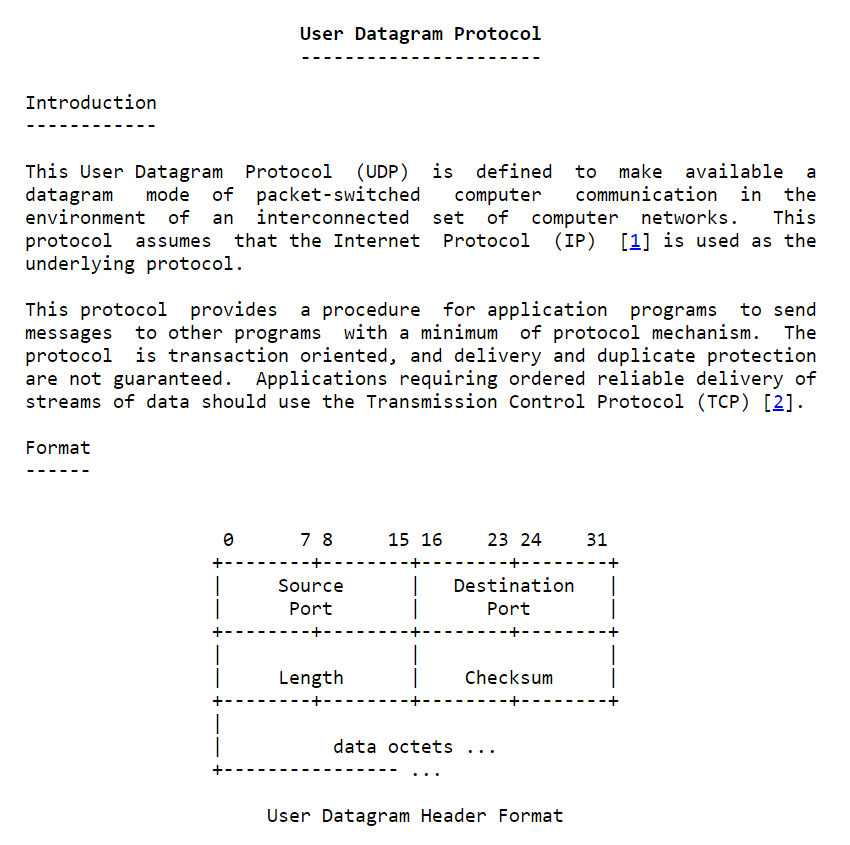
\includegraphics[height=300px]{images/UDP.PNG}
                \end{center}
        \item \textbf{UDP datagrams} have the following headers:
        \begin{enumerate}
            \item \textbf{Destination port} | The port the datagram is being sent to.
            \item \textbf{Length} | The length in octets of the datagram.
            \item \textbf{Checksum} | The checksum is used to ensure the packet received was not corrupted during transmission.
            \item \textbf{Pseudo} | A header containing the source address, destination address, the protocol, and the UDP length. This information is used to give protection against misrouted datagrams.
        \end{enumerate} 
        \item The \textbf{checksum} is computed by taking the \textbf{one's complement sum} of the \textbf{entire content} of the \textbf{datagram}, treating the bits of the datagram as a \textbf{series of 16-bit integers}.
        \begin{itemize}
            \item The checksum is not perfect, several different datagrams can result in the same checksum.
        \end{itemize}
    \end{itemize}

    \section*{Reliable Data Transfer}

\end{document}